\section{Proposed Soluction}

We propose to bridge the adaptable component-base architectures research field with goal-model by making central to the platform the concept of 'strategy' both a mean of achieving a goal (as in goal-based RE) and a component in the architecture. By this we aim at creating an appropriate abstraction to allow composable adaptable architecture while keeping the traceability between the requirements and implementation at runtime.

We propose a middleware support for self-adaptable capable of keep the traceability between goals and architecture.

That middleware should have a simple programming model and be flexible so that further domains specific applications and frameworks can be build on top of it.

The middleware will be open-source, reasonably documented in its use and development process. By this we pretend allow for future validation of effective use.

\begin{comment}

Finally we explore how to use the middleware support for development of distributed, open-adaptable, opportunistic and evolvable application.

As a support for open-systems, we propose a multi-agent approach in witch agents can collaborate by making peer agents 'strategies' discoverable.

\begin{figure}
  \centering
  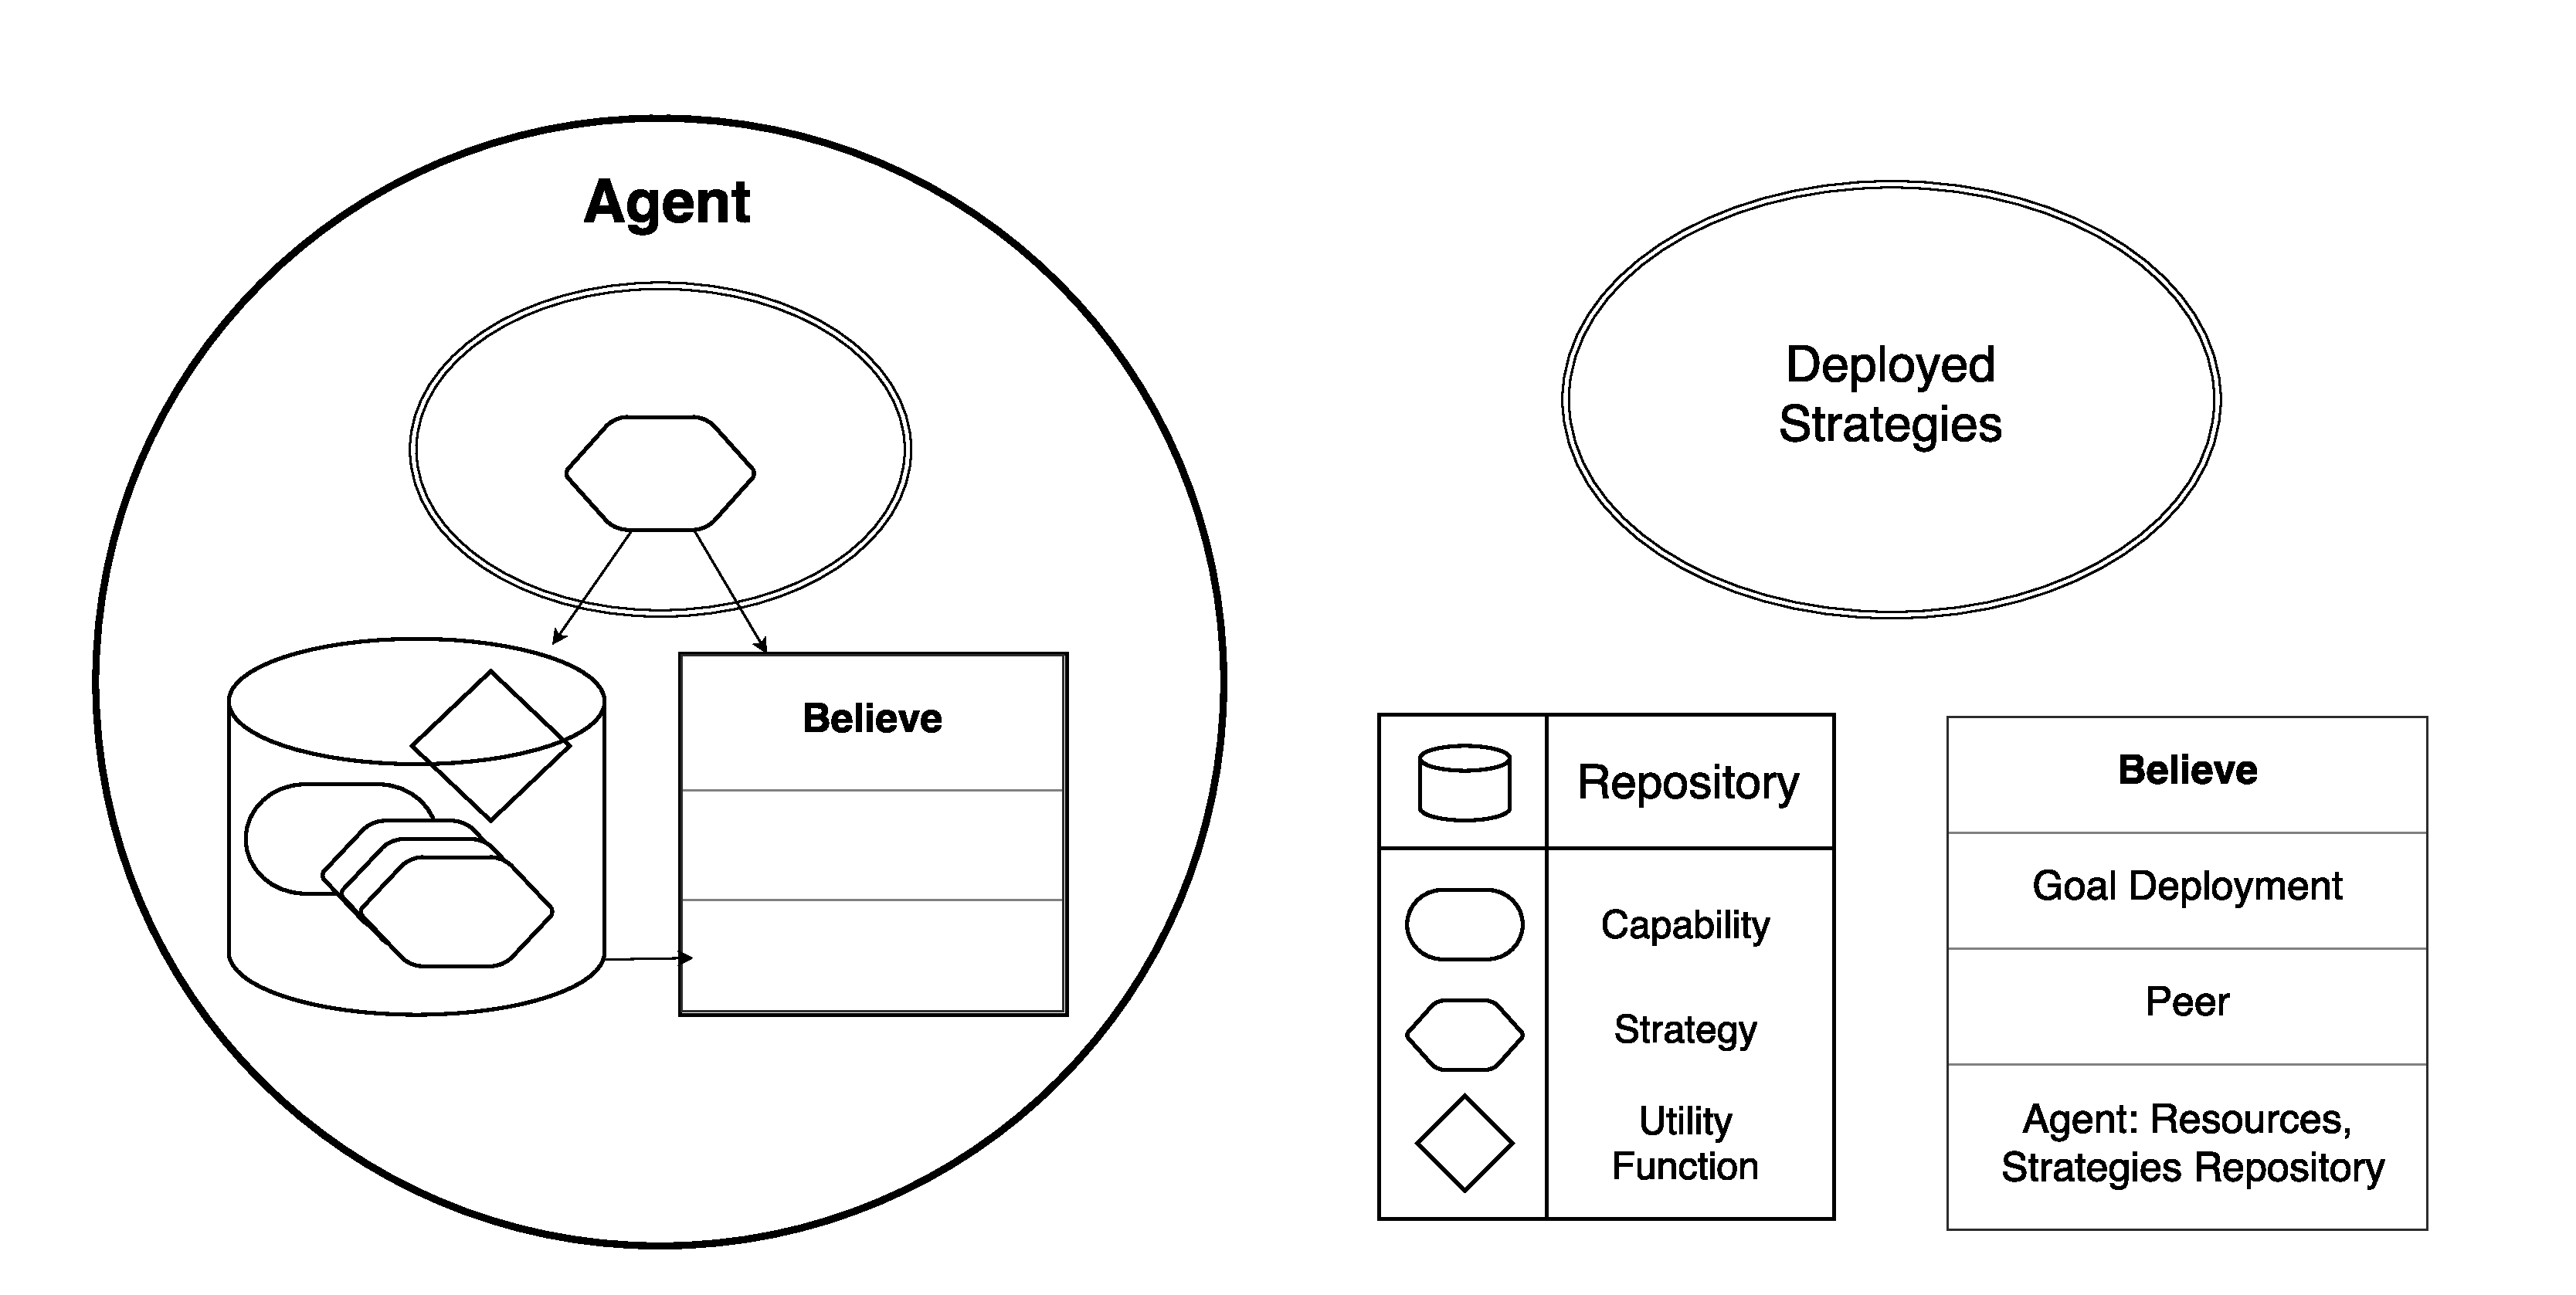
\includegraphics[width=\linewidth]{goalp-agent-repo-rcm-depl}
  \caption{The proposed agent composition}
  \label{fig:agent_composition}
\end{figure}

We followend an approach with run-time goal model with an mechanism for compositional adaptation and multi-agent collaboration. In our propose adaptiveness is achived by means of strategies matching an selection at runtime. For more flexibility we propose a symetric design.

By composable simetry we mean that we should be able to compose strategies in new strategies, and made agents out of strategies and teams out of agents. All with the same interface, transparent for a peer client.

\end{comment}

%\subsection{Evaluation}
